\par\vspace{3mm}
{\large \textbf{Custom Search Results Header:}}

In this section, users can interact with various features for downloading, viewing, and interacting with the results:
\begin{figure}[H]
  \centering  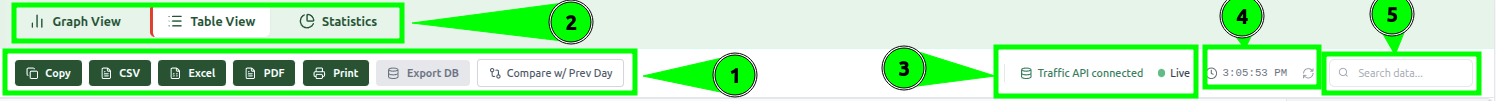
\includegraphics[width=\textwidth]{img/common/commonarea/results/ResultsCommonArea.png}

  \caption{Example of Results Common Area}
\end{figure}
\begin{enumerate}
  \item \textbf{Download and Export Options:}
    Users can download the custom results in different formats such as \textbf{CSV}, \textbf{Excel}, \textbf{PDF}, or \textbf{Copy}, or they can choose to print the results. Additionally, users can export the data directly from the database and compare it with the previous day's data.

  \item \textbf{View Options:}
    Users can view the results in different modes:
    \begin{itemize}
      \item Graph View – Display the results in a graphical format.
      \item Table View – View the results in a tabular format.
      \item Statistics – View the detailed statistics.
    \end{itemize}

  \item \textbf{Traffic API Status:}
    It is crucial to check whether the \textbf{Traffic API} is connected. If the API is disconnected, data may not load, and the user might not be able to view the required results.

  \item \textbf{Server Time:}
    The \textbf{Server Time} is displayed to indicate the current time of the server, which can be useful for comparing time-sensitive data.

  \item \textbf{Search Area:}
    The user can utilize the \textbf{Search Area} to search for specific data within the results table.
\end{enumerate}
